% Options for packages loaded elsewhere
\PassOptionsToPackage{unicode}{hyperref}
\PassOptionsToPackage{hyphens}{url}
%
\documentclass[
]{article}
\usepackage{amsmath,amssymb}
\usepackage{lmodern}
\usepackage{iftex}
\ifPDFTeX
  \usepackage[T1]{fontenc}
  \usepackage[utf8]{inputenc}
  \usepackage{textcomp} % provide euro and other symbols
\else % if luatex or xetex
  \usepackage{unicode-math}
  \defaultfontfeatures{Scale=MatchLowercase}
  \defaultfontfeatures[\rmfamily]{Ligatures=TeX,Scale=1}
\fi
% Use upquote if available, for straight quotes in verbatim environments
\IfFileExists{upquote.sty}{\usepackage{upquote}}{}
\IfFileExists{microtype.sty}{% use microtype if available
  \usepackage[]{microtype}
  \UseMicrotypeSet[protrusion]{basicmath} % disable protrusion for tt fonts
}{}
\makeatletter
\@ifundefined{KOMAClassName}{% if non-KOMA class
  \IfFileExists{parskip.sty}{%
    \usepackage{parskip}
  }{% else
    \setlength{\parindent}{0pt}
    \setlength{\parskip}{6pt plus 2pt minus 1pt}}
}{% if KOMA class
  \KOMAoptions{parskip=half}}
\makeatother
\usepackage{xcolor}
\IfFileExists{xurl.sty}{\usepackage{xurl}}{} % add URL line breaks if available
\IfFileExists{bookmark.sty}{\usepackage{bookmark}}{\usepackage{hyperref}}
\hypersetup{
  pdftitle={Homework 2},
  pdfauthor={Maya Sinha},
  hidelinks,
  pdfcreator={LaTeX via pandoc}}
\urlstyle{same} % disable monospaced font for URLs
\usepackage[margin=1in]{geometry}
\usepackage{color}
\usepackage{fancyvrb}
\newcommand{\VerbBar}{|}
\newcommand{\VERB}{\Verb[commandchars=\\\{\}]}
\DefineVerbatimEnvironment{Highlighting}{Verbatim}{commandchars=\\\{\}}
% Add ',fontsize=\small' for more characters per line
\usepackage{framed}
\definecolor{shadecolor}{RGB}{248,248,248}
\newenvironment{Shaded}{\begin{snugshade}}{\end{snugshade}}
\newcommand{\AlertTok}[1]{\textcolor[rgb]{0.94,0.16,0.16}{#1}}
\newcommand{\AnnotationTok}[1]{\textcolor[rgb]{0.56,0.35,0.01}{\textbf{\textit{#1}}}}
\newcommand{\AttributeTok}[1]{\textcolor[rgb]{0.77,0.63,0.00}{#1}}
\newcommand{\BaseNTok}[1]{\textcolor[rgb]{0.00,0.00,0.81}{#1}}
\newcommand{\BuiltInTok}[1]{#1}
\newcommand{\CharTok}[1]{\textcolor[rgb]{0.31,0.60,0.02}{#1}}
\newcommand{\CommentTok}[1]{\textcolor[rgb]{0.56,0.35,0.01}{\textit{#1}}}
\newcommand{\CommentVarTok}[1]{\textcolor[rgb]{0.56,0.35,0.01}{\textbf{\textit{#1}}}}
\newcommand{\ConstantTok}[1]{\textcolor[rgb]{0.00,0.00,0.00}{#1}}
\newcommand{\ControlFlowTok}[1]{\textcolor[rgb]{0.13,0.29,0.53}{\textbf{#1}}}
\newcommand{\DataTypeTok}[1]{\textcolor[rgb]{0.13,0.29,0.53}{#1}}
\newcommand{\DecValTok}[1]{\textcolor[rgb]{0.00,0.00,0.81}{#1}}
\newcommand{\DocumentationTok}[1]{\textcolor[rgb]{0.56,0.35,0.01}{\textbf{\textit{#1}}}}
\newcommand{\ErrorTok}[1]{\textcolor[rgb]{0.64,0.00,0.00}{\textbf{#1}}}
\newcommand{\ExtensionTok}[1]{#1}
\newcommand{\FloatTok}[1]{\textcolor[rgb]{0.00,0.00,0.81}{#1}}
\newcommand{\FunctionTok}[1]{\textcolor[rgb]{0.00,0.00,0.00}{#1}}
\newcommand{\ImportTok}[1]{#1}
\newcommand{\InformationTok}[1]{\textcolor[rgb]{0.56,0.35,0.01}{\textbf{\textit{#1}}}}
\newcommand{\KeywordTok}[1]{\textcolor[rgb]{0.13,0.29,0.53}{\textbf{#1}}}
\newcommand{\NormalTok}[1]{#1}
\newcommand{\OperatorTok}[1]{\textcolor[rgb]{0.81,0.36,0.00}{\textbf{#1}}}
\newcommand{\OtherTok}[1]{\textcolor[rgb]{0.56,0.35,0.01}{#1}}
\newcommand{\PreprocessorTok}[1]{\textcolor[rgb]{0.56,0.35,0.01}{\textit{#1}}}
\newcommand{\RegionMarkerTok}[1]{#1}
\newcommand{\SpecialCharTok}[1]{\textcolor[rgb]{0.00,0.00,0.00}{#1}}
\newcommand{\SpecialStringTok}[1]{\textcolor[rgb]{0.31,0.60,0.02}{#1}}
\newcommand{\StringTok}[1]{\textcolor[rgb]{0.31,0.60,0.02}{#1}}
\newcommand{\VariableTok}[1]{\textcolor[rgb]{0.00,0.00,0.00}{#1}}
\newcommand{\VerbatimStringTok}[1]{\textcolor[rgb]{0.31,0.60,0.02}{#1}}
\newcommand{\WarningTok}[1]{\textcolor[rgb]{0.56,0.35,0.01}{\textbf{\textit{#1}}}}
\usepackage{graphicx}
\makeatletter
\def\maxwidth{\ifdim\Gin@nat@width>\linewidth\linewidth\else\Gin@nat@width\fi}
\def\maxheight{\ifdim\Gin@nat@height>\textheight\textheight\else\Gin@nat@height\fi}
\makeatother
% Scale images if necessary, so that they will not overflow the page
% margins by default, and it is still possible to overwrite the defaults
% using explicit options in \includegraphics[width, height, ...]{}
\setkeys{Gin}{width=\maxwidth,height=\maxheight,keepaspectratio}
% Set default figure placement to htbp
\makeatletter
\def\fps@figure{htbp}
\makeatother
\setlength{\emergencystretch}{3em} % prevent overfull lines
\providecommand{\tightlist}{%
  \setlength{\itemsep}{0pt}\setlength{\parskip}{0pt}}
\setcounter{secnumdepth}{-\maxdimen} % remove section numbering
\ifLuaTeX
  \usepackage{selnolig}  % disable illegal ligatures
\fi

\title{Homework 2}
\author{Maya Sinha}
\date{2022-10-06}

\begin{document}
\maketitle

\hypertarget{question-1}{%
\subsubsection{Question 1}\label{question-1}}

\begin{Shaded}
\begin{Highlighting}[]
\FunctionTok{setwd}\NormalTok{(}\StringTok{"/Users/mayasinha/Desktop/PSTAT 131/homework{-}2/data"}\NormalTok{) }
\FunctionTok{getwd}\NormalTok{()}
\end{Highlighting}
\end{Shaded}

\begin{verbatim}
## [1] "/Users/mayasinha/Desktop/PSTAT 131/homework-2/data"
\end{verbatim}

\begin{Shaded}
\begin{Highlighting}[]
\NormalTok{abalone\_df }\OtherTok{\textless{}{-}} \FunctionTok{read\_csv}\NormalTok{(}\StringTok{"abalone.csv"}\NormalTok{)}
\NormalTok{age }\OtherTok{\textless{}{-}}\NormalTok{ abalone\_df[,}\DecValTok{9}\NormalTok{]}\SpecialCharTok{+}\FloatTok{1.5}
\NormalTok{abalone\_df }\OtherTok{\textless{}{-}} \FunctionTok{cbind}\NormalTok{(abalone\_df, age)}
\FunctionTok{names}\NormalTok{(abalone\_df)[}\DecValTok{10}\NormalTok{] }\OtherTok{\textless{}{-}} \StringTok{"age"}
\NormalTok{abalone\_df }\SpecialCharTok{\%\textgreater{}\%} 
  \FunctionTok{ggplot}\NormalTok{(}\FunctionTok{aes}\NormalTok{(}\AttributeTok{x =}\NormalTok{ age)) }\SpecialCharTok{+}
  \FunctionTok{geom\_histogram}\NormalTok{(}\AttributeTok{bins =} \DecValTok{60}\NormalTok{) }
\end{Highlighting}
\end{Shaded}

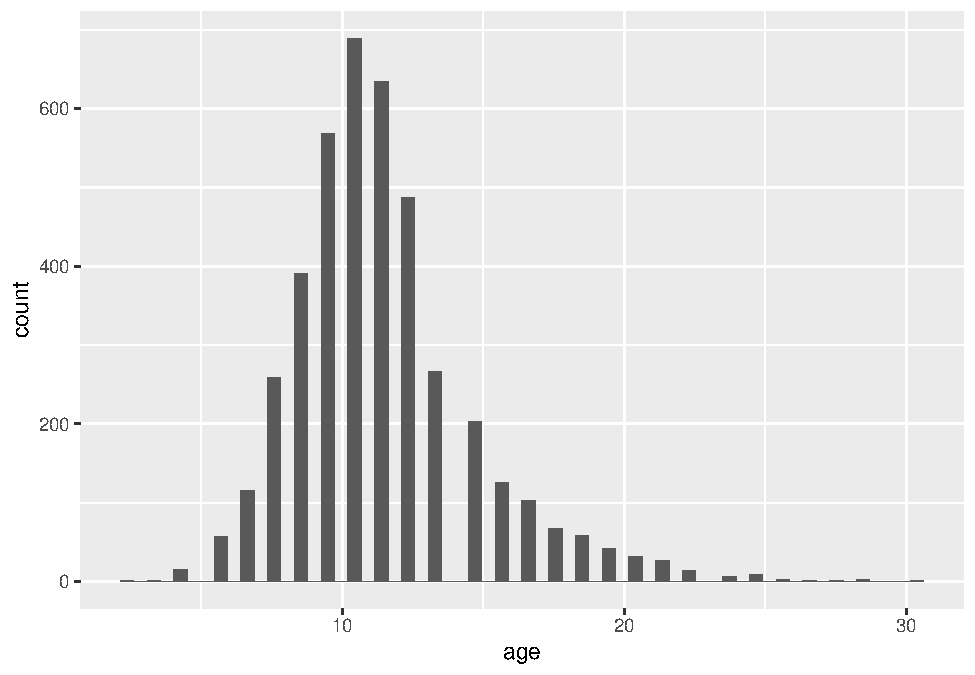
\includegraphics{Homework-2_files/figure-latex/unnamed-chunk-2-1.pdf}

Age seems to have normal distribution with a slight right skewed nature.

\hypertarget{question-2}{%
\subsubsection{Question 2}\label{question-2}}

\begin{Shaded}
\begin{Highlighting}[]
\FunctionTok{set.seed}\NormalTok{(}\DecValTok{1215}\NormalTok{)}

\NormalTok{abalone\_split }\OtherTok{\textless{}{-}} \FunctionTok{initial\_split}\NormalTok{(abalone\_df, }\AttributeTok{prop =}\NormalTok{ .}\DecValTok{75}\NormalTok{, }\AttributeTok{strata =}\NormalTok{ age)}
\NormalTok{abalone\_train }\OtherTok{\textless{}{-}} \FunctionTok{training}\NormalTok{(abalone\_split)}
\NormalTok{abalone\_test }\OtherTok{\textless{}{-}} \FunctionTok{testing}\NormalTok{(abalone\_split)}
\end{Highlighting}
\end{Shaded}

\hypertarget{question-3}{%
\subsubsection{Question 3}\label{question-3}}

\begin{Shaded}
\begin{Highlighting}[]
\NormalTok{abalone\_recipe }\OtherTok{\textless{}{-}} \FunctionTok{recipe}\NormalTok{(age }\SpecialCharTok{\textasciitilde{}}\NormalTok{ type }\SpecialCharTok{+}\NormalTok{ longest\_shell }\SpecialCharTok{+}\NormalTok{ diameter }\SpecialCharTok{+}\NormalTok{ height }\SpecialCharTok{+}\NormalTok{   whole\_weight }\SpecialCharTok{+}\NormalTok{ shucked\_weight }\SpecialCharTok{+}\NormalTok{ viscera\_weight  }\SpecialCharTok{+}\NormalTok{ shell\_weight, }\AttributeTok{data =}\NormalTok{ abalone\_train) }\SpecialCharTok{\%\textgreater{}\%} 
  \FunctionTok{step\_dummy}\NormalTok{(}\FunctionTok{all\_nominal\_predictors}\NormalTok{()) }\SpecialCharTok{\%\textgreater{}\%} 
  \FunctionTok{step\_interact}\NormalTok{(}\AttributeTok{terms =} \SpecialCharTok{\textasciitilde{}} \FunctionTok{starts\_with}\NormalTok{(}\StringTok{"type"}\NormalTok{)}\SpecialCharTok{:}\NormalTok{shucked\_weight }\SpecialCharTok{+}\NormalTok{ longest\_shell}\SpecialCharTok{:}\NormalTok{diameter }\SpecialCharTok{+}\NormalTok{ shucked\_weight}\SpecialCharTok{:}\NormalTok{shell\_weight) }\SpecialCharTok{\%\textgreater{}\%} 
  \FunctionTok{step\_center}\NormalTok{(}\FunctionTok{all\_predictors}\NormalTok{()) }\SpecialCharTok{\%\textgreater{}\%} 
  \FunctionTok{step\_scale}\NormalTok{(}\FunctionTok{all\_predictors}\NormalTok{())}

\NormalTok{abalone\_recipe}
\end{Highlighting}
\end{Shaded}

\begin{verbatim}
## Recipe
## 
## Inputs:
## 
##       role #variables
##    outcome          1
##  predictor          8
## 
## Operations:
## 
## Dummy variables from all_nominal_predictors()
## Interactions with starts_with("type"):shucked_weight + longest_shell...
## Centering for all_predictors()
## Scaling for all_predictors()
\end{verbatim}

We do not use rings to predict age because age is directly based on
rings (age = 1.5 * number of rings).

\hypertarget{question-4}{%
\subsubsection{Question 4}\label{question-4}}

\begin{Shaded}
\begin{Highlighting}[]
\NormalTok{lm\_model }\OtherTok{\textless{}{-}} \FunctionTok{linear\_reg}\NormalTok{() }\SpecialCharTok{\%\textgreater{}\%} 
  \FunctionTok{set\_engine}\NormalTok{(}\StringTok{"lm"}\NormalTok{)}
\end{Highlighting}
\end{Shaded}

\hypertarget{question-5}{%
\subsubsection{Question 5}\label{question-5}}

\begin{Shaded}
\begin{Highlighting}[]
\NormalTok{lm\_wflow }\OtherTok{\textless{}{-}} \FunctionTok{workflow}\NormalTok{() }\SpecialCharTok{\%\textgreater{}\%} 
  \FunctionTok{add\_model}\NormalTok{(lm\_model) }\SpecialCharTok{\%\textgreater{}\%} 
  \FunctionTok{add\_recipe}\NormalTok{(abalone\_recipe)}
\end{Highlighting}
\end{Shaded}

\hypertarget{question-6}{%
\subsubsection{Question 6}\label{question-6}}

\begin{Shaded}
\begin{Highlighting}[]
\NormalTok{abalone\_fit }\OtherTok{\textless{}{-}} \FunctionTok{fit}\NormalTok{(lm\_wflow, abalone\_train)}
\NormalTok{abalone\_fit }\SpecialCharTok{\%\textgreater{}\%} \FunctionTok{extract\_fit\_parsnip}\NormalTok{() }\SpecialCharTok{\%\textgreater{}\%} \FunctionTok{tidy}\NormalTok{()}
\end{Highlighting}
\end{Shaded}

\begin{verbatim}
## # A tibble: 14 x 5
##    term                          estimate std.error statistic  p.value
##    <chr>                            <dbl>     <dbl>     <dbl>    <dbl>
##  1 (Intercept)                    11.4       0.0383   298.    0       
##  2 longest_shell                   0.388     0.302      1.29  1.98e- 1
##  3 diameter                        2.74      0.330      8.29  1.73e-16
##  4 height                          0.227     0.0713     3.18  1.50e- 3
##  5 whole_weight                    5.40      0.419     12.9   4.18e-37
##  6 shucked_weight                 -4.51      0.262    -17.2   1.55e-63
##  7 viscera_weight                 -0.921     0.165     -5.58  2.63e- 8
##  8 shell_weight                    1.42      0.219      6.48  1.08e-10
##  9 type_I                         -0.897     0.118     -7.59  4.17e-14
## 10 type_M                         -0.257     0.107     -2.40  1.66e- 2
## 11 type_I_x_shucked_weight         0.503     0.0884     5.70  1.34e- 8
## 12 type_M_x_shucked_weight         0.377     0.114      3.31  9.27e- 4
## 13 longest_shell_x_diameter       -3.38      0.423     -8.00  1.71e-15
## 14 shucked_weight_x_shell_weight  -0.0665    0.209     -0.318 7.51e- 1
\end{verbatim}

\begin{Shaded}
\begin{Highlighting}[]
\NormalTok{abalone\_fit}
\end{Highlighting}
\end{Shaded}

\begin{verbatim}
## == Workflow [trained] ==========================================================
## Preprocessor: Recipe
## Model: linear_reg()
## 
## -- Preprocessor ----------------------------------------------------------------
## 4 Recipe Steps
## 
## * step_dummy()
## * step_interact()
## * step_center()
## * step_scale()
## 
## -- Model -----------------------------------------------------------------------
## 
## Call:
## stats::lm(formula = ..y ~ ., data = data)
## 
## Coefficients:
##                   (Intercept)                  longest_shell  
##                      11.43389                        0.38787  
##                      diameter                         height  
##                       2.73792                        0.22670  
##                  whole_weight                 shucked_weight  
##                       5.39961                       -4.50661  
##                viscera_weight                   shell_weight  
##                      -0.92143                        1.41659  
##                        type_I                         type_M  
##                      -0.89675                       -0.25695  
##       type_I_x_shucked_weight        type_M_x_shucked_weight  
##                       0.50329                        0.37657  
##      longest_shell_x_diameter  shucked_weight_x_shell_weight  
##                      -3.38185                       -0.06648
\end{verbatim}

\begin{Shaded}
\begin{Highlighting}[]
\NormalTok{new\_abalone }\OtherTok{\textless{}{-}} \FunctionTok{tibble}\NormalTok{(}\AttributeTok{type =} \StringTok{"F"}\NormalTok{, }\AttributeTok{longest\_shell =} \FloatTok{0.50}\NormalTok{, }\AttributeTok{diameter =} \FloatTok{0.1}\NormalTok{, }\AttributeTok{height =} \FloatTok{0.3}\NormalTok{, }\AttributeTok{whole\_weight =} \DecValTok{4}\NormalTok{, }\AttributeTok{shucked\_weight =} \DecValTok{1}\NormalTok{, }\AttributeTok{viscera\_weight =} \DecValTok{2}\NormalTok{, }\AttributeTok{shell\_weight =} \DecValTok{1}\NormalTok{, }\AttributeTok{rings =} \DecValTok{0}\NormalTok{)}
\FunctionTok{predict}\NormalTok{(abalone\_fit, }\AttributeTok{new\_data =}\NormalTok{ new\_abalone)}
\end{Highlighting}
\end{Shaded}

\begin{verbatim}
## # A tibble: 1 x 1
##   .pred
##   <dbl>
## 1  24.1
\end{verbatim}

\hypertarget{question-7}{%
\subsubsection{Question 7}\label{question-7}}

\begin{Shaded}
\begin{Highlighting}[]
\NormalTok{abalone\_train\_res }\OtherTok{\textless{}{-}} \FunctionTok{predict}\NormalTok{(abalone\_fit, }\AttributeTok{new\_data =}\NormalTok{ abalone\_train }\SpecialCharTok{\%\textgreater{}\%} \FunctionTok{select}\NormalTok{(}\SpecialCharTok{{-}}\NormalTok{age))}
\NormalTok{abalone\_train\_res }\OtherTok{\textless{}{-}} \FunctionTok{bind\_cols}\NormalTok{(abalone\_train\_res, abalone\_train }\SpecialCharTok{\%\textgreater{}\%} \FunctionTok{select}\NormalTok{(age))}


\NormalTok{abalone\_metrics }\OtherTok{\textless{}{-}} \FunctionTok{metric\_set}\NormalTok{(rmse, rsq, mae)}
\FunctionTok{abalone\_metrics}\NormalTok{(abalone\_train\_res, }\AttributeTok{truth =}\NormalTok{ age, }
                \AttributeTok{estimate =}\NormalTok{ .pred)}
\end{Highlighting}
\end{Shaded}

\begin{verbatim}
## # A tibble: 3 x 3
##   .metric .estimator .estimate
##   <chr>   <chr>          <dbl>
## 1 rmse    standard       2.14 
## 2 rsq     standard       0.562
## 3 mae     standard       1.54
\end{verbatim}

interpret

\end{document}
